\chapter{Einleitung}
Dieses Manual bietet eine Anleitung für den Benutzer zur Verwendung des
Multicast Test Tools. Dabei richtet sich dieses Dokument an fortgeschrittene
Benutzer, die mit der Funktionalität von Multicast vertraut sind, sowie
hinreichende Kenntnisse im Umgang mit Computern und Programmen mit
grafischer Benutzeroberfläche besitzen. Im Folgenden wird dafür auf die
einzelnen Fenster/Dialoge des Programmes eingegangen und deren Funktionalität kurz erläutert.
  
\chapter{Übersicht Hauptfenster}

Das Hauptfenster des Multicast Test Tools besteht aus einem Menü, der
Senderliste, der Empfängerliste und jeweils rechts der beiden Listen globale
Statistiken zu allen Sendern bzw. Empfängern.

\begin{figure}[htbp]
\begin{center}
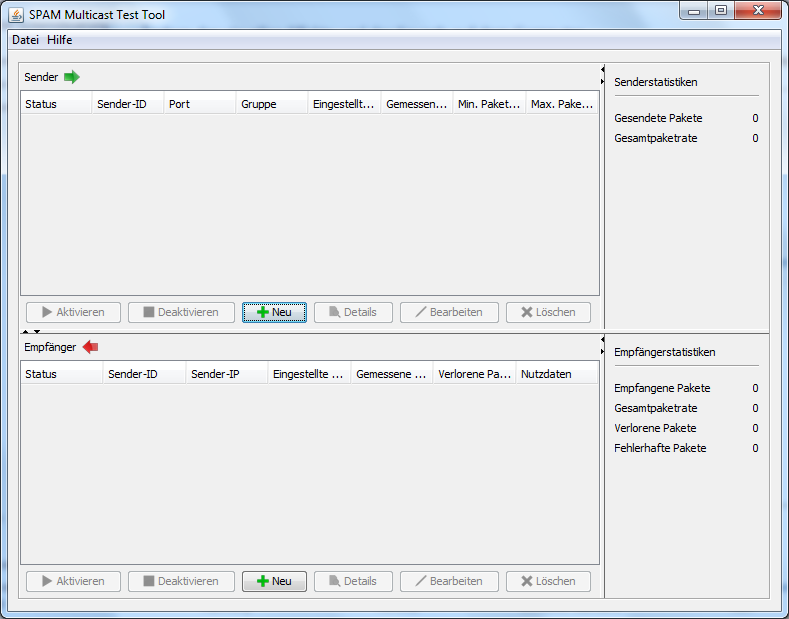
\includegraphics[width=14cm]{images/mainFrameBasic.png}
\caption[GUI Übersicht]{GUI Übersicht}
\label{overview}
\end{center}
\end{figure}

Die Sender und Empfänger werden nach Anlegen in der jeweiligen Liste zusammen
mit einigen sender- bzw. empfängerspezifischen Statistiken in der Liste
angezeigt.

\begin{figure}[htbp]
\begin{center}
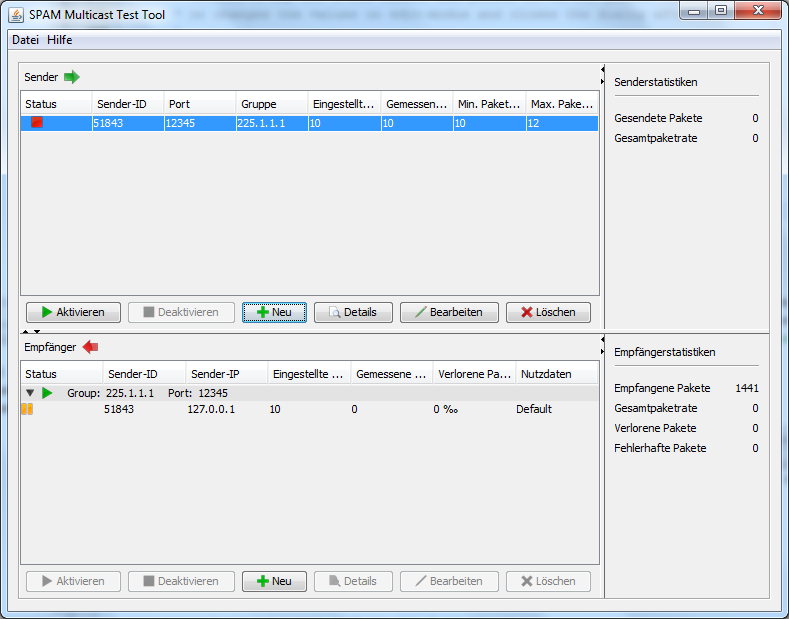
\includegraphics[width=14cm]{images/mainFrameDeactivateSender.png}
\caption[GUI Übersicht - 2]{GUI Übersicht - 2}
\label{overview}
\end{center}
\end{figure}

Einer oder mehrere bereits existierende Sender oder Empfänger können nach
Auswahl in der entsprechenden Liste durch einen einfachen Klick auf ``Aktivieren''
aktiviert bzw. ``Deaktivieren'' deaktiviert werden. Aktivierte
Sender/Empfänger sind durch einen grünen Pfeil gekennzeichnet, deaktivierte
durch ein rotes Quadrat.
\newline
Eine Empfänger kann mehrere Multicast-Streams empfangen, die auf die gleiche
Gruppe gesendet werden. Diese werden in einer Liste unterhalb des
Empfängers angezeigt. Wenn von einem der Streams keine Pakete mehr empfangen
werden, so wird dieser durch ein gelbes ``Pause''-Zeichen gekennzeichnet.
\newline
Ein Klick auf ``Löschen'' oder ein Drücken des ``Entf''-Knopfes auf der Tastatur
entfernt die jeweils ausgewählten Einträge aus der Liste.

\chapter{Neuer Sender}
Zum Anlegen eines Senders ist unterhalb der Senderliste
ein Button vorhanden mit der Aufschrift ``Neu''. Durch einen Klick auf diesen
Button wird ein Dialogfenster geöffnet.

\begin{figure}[htbp]
\begin{center}
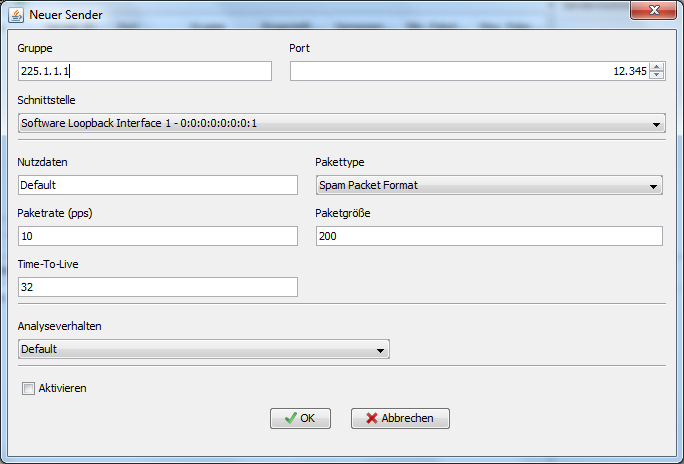
\includegraphics[width=14cm]{images/addSender.png}
\caption[Neuer Sender]{Neuer Sender}
\label{newSender}
\end{center}
\end{figure}

Innerhalb dieses Dialogfensters sind verschiedene Felder zur Konfiguration des
Senders vorhanden. Die meisten der Felder enthalten bereits einen Standardwert.
Hierbei ist anzumerken, dass bei klicken auf den ``Neu''-Button mit aktuell
ausgewähltem Sender die Konfiguration des ausgewählten
Senders im ``Neuer Sender"-Dialog voreingetragen wird.

\begin{table}[h]
\caption{Eingabefelder - Neuer Sender}
\label{tab:inputNewSender}
\begin{center}
\begin{tabular}{|l|p{10cm}|}
\hline
\textbf{Bezeichnung} & \textbf{Beschreibung}\\
\hline
Gruppe & Definiert die IP der Multicast-Gruppe\\
\hline
Port & Definiert den Port der Multicast-Gruppe\\
\hline
Schnittstelle & Definiert welcher Netzwerk-Adapter verwendet werden soll\\
\hline
Nutzdaten & Definiert den Textstring, der im Paket mitgesendet werden soll\\
\hline
Pakettyp & Definiert den Pakettyp. (Hirschmann/SPAM)\\
\hline
Paketrate & Definiert die Anzahl der Pakete, die pro Sekunde verschickt werden\\
\hline
Paketgröße & Definiert die Größe eines Pakets\\
\hline
Time-To-Live & Definiert, wie lange ein Paket maximal im Netzwerk unterwegs sein
darf\\
\hline
Analyseverhalten & Definiert das Analyseverhalten/die Häufigkeit der
Statistikberechnung\\
\hline
 Aktivieren & Aktiviert den Sender direkt nach Anlegen\\
\hline
\end{tabular}
\end{center}
\label{default}
\end{table}

\chapter{Sender bearbeiten}
Zum Bearbeiten eines Senders ist unterhalb der Senderliste
ein Button vorhanden mit der Aufschrift ``Bearbeiten''. Durch einen Klick auf
diesen Button bei ausgewähltem/markiertem Sender wird ein Dialogfenster
geöffnet.

\begin{figure}[htbp]
\begin{center}
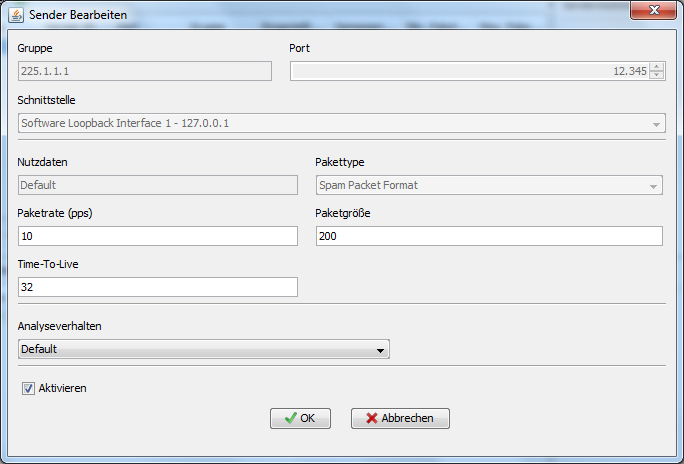
\includegraphics[width=14cm]{images/editSender.png}
\caption[Sender bearbeiten]{Sender bearbeiten}
\label{newReceiver}
\end{center}
\end{figure}

Innerhalb dieses Dialogfensters sind verschiedene Felder zum Bearbeiten des
Senders vorhanden. Die inaktiven Felder dienen hier zur Orientierung, es ist
jedoch nicht erlaubt diese zu bearbeiten. Lediglich die aktiven Felder sind
bearbeitbar.

\begin{table}[h]
\caption{Eingabefelder - Sender bearbeiten}
\label{tab:inputEditSender}
\begin{center}
\begin{tabular}{|l|p{10cm}|}
\hline
\textbf{Bezeichnung} & \textbf{Beschreibung}\\
\hline
Pakettyp & Definiert den Pakettyp. (Hirschmann/SPAM)\\
\hline
Paketrate & Definiert die Anzahl der Pakete, die pro Sekunde verschickt werden\\
\hline
Paketgröße & Definiert die Größe eines Pakets\\
\hline
Time-To-Live & Definiert, wie lange ein Paket maximal im Netzwerk unterwegs sein
darf\\
\hline
Analyseverhalten & Definiert das Analyseverhalten/die Häufigkeit der
Statistikberechnung\\
\hline
 Aktivieren & Aktiviert den Sender direkt nach Anlegen\\
\hline
\end{tabular}
\end{center}
\label{default}
\end{table}

\chapter{Senderstatistiken}
Zum Anzeigen der Statistiken eines Senders ist unterhalb der Senderliste ein
Button vorhanden mit der Aufschrift ``Details''. Ein Klick auf diesen Button
öffnet ein Dialogfenster.

\begin{figure}[htbp]
\begin{center}
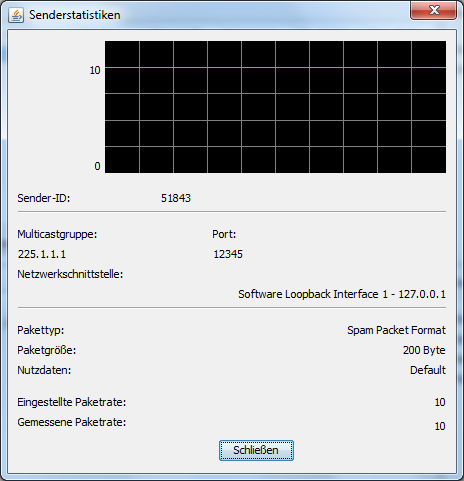
\includegraphics{images/showSender.png}
\caption[Senderstatistiken]{Senderstatistiken}
\label{senderstatistics}
\end{center}
\end{figure}

Innerhalb dieses Dialogfensters werden verschiedene Statistiken, allgemeine
Informationen zum Sender, sowie ein Graph, welcher den Verlauf der Paketrate
darstellt, angezeigt.

\begin{table}[h]
\caption{Daten - Senderstatistiken}
\label{tab:showSender}
\begin{center}
\begin{tabular}{|l|p{10cm}|}
\hline
\textbf{Bezeichnung} & \textbf{Beschreibung}\\
\hline
Graph & Zeigt grafisch den Verlauf der gemessenen Paketrate\\
\hline
Sender-ID & Zeigt die Sender-ID an\\
\hline
Multicastgruppe & Zeigt die Multicastgruppe, an die gesendet wird.\\
\hline
Port & Zeigt den Port, an den gesendet wird\\
\hline
Pakettyp & Zeigt den verwendeten Pakettypen\\
\hline
Paketgröße & Zeigt die definierte Paketgröße\\
\hline
Nutzdaten & Zeigt die definierten Nutzdaten\\
\hline
Eingestellte Paketrate & Zeigt die eingestellte Paketrate\\
\hline
Gemessene Paketrate & Zeigt die gemessene Paketrate\\
\hline
\end{tabular}
\end{center}
\label{default}
\end{table}


\chapter{Neuer Empfänger}
Zum Anlegen eines Empfängers ist unterhalb der Empfängerliste
ein Button vorhanden mit der Aufschrift ``Neu''. Durch einen Klick auf diesen
Button wird ein Dialogfenster geöffnet.

\begin{figure}[htbp]
\begin{center}
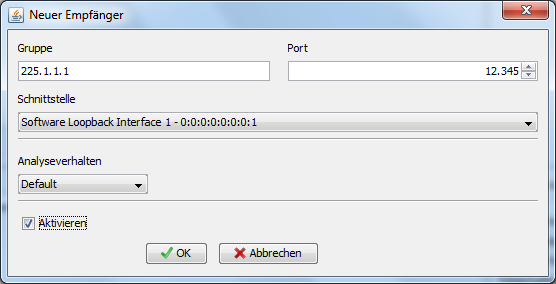
\includegraphics[width=14cm]{images/addEmpfaenger.png}
\caption[Neuer Empfänger]{Neuer Empfänger}
\label{newSender}
\end{center}
\end{figure}

Innerhalb dieses Dialogfensters sind verschiedene Felder zur Konfiguration des
Empfängers vorhanden. Die meisten der Felder enthalten bereits einen
Standardwert. Hierbei ist anzumerken, dass bei klicken auf den ``Neu''-Button mit aktuell
ausgewähltem Empfänger die Konfiguration des ausgewählten
Empfängers im ``Neuer Empfänger''-Dialog voreingetragen wird.

\begin{table}[h]
\caption{Eingabefelder - Neuer Empfänger}
\label{tab:inputNewSender}
\begin{center}
\begin{tabular}{|l|p{10cm}|}
\hline
\textbf{Bezeichnung} & \textbf{Beschreibung}\\
\hline
Gruppe & Definiert die IP der Multicast-Gruppe\\
\hline
Port & Definiert den Port der Multicast-Gruppe\\
\hline
Schnittstelle & Definiert welcher Netzwerk-Adapter verwendet werden soll\\
\hline
Analyseverhalten & Definiert das Analyseverhalten/die Häufigkeit der
Statistikberechnung\\
\hline
 Aktivieren & Aktiviert den Sender direkt nach Anlegen\\
\hline
\end{tabular}
\end{center}
\label{default}
\end{table}

\chapter{Empfänger bearbeiten}
Zum Bearbeiten eines Empfängers ist unterhalb der Empfängerliste
ein Button vorhanden mit der Aufschrift ``Bearbeiten''. Durch einen Klick auf
diesen Button bei ausgewähltem/markiertem Sender wird ein Dialogfenster
geöffnet.

\begin{figure}[htbp]
\begin{center}
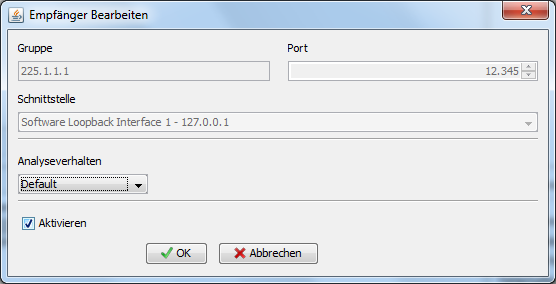
\includegraphics[width=14cm]{images/editEmpfaenger.png}
\caption[Empfänger bearbeiten]{Empfänger bearbeiten}
\label{newReceiver}
\end{center}
\end{figure}

Innerhalb dieses Dialogfensters sind verschiedene Felder zum Bearbeiten des
Empfängers vorhanden. Die inaktiven Felder dienen hier zur Orientierung, es ist
jedoch nicht erlaubt diese zu bearbeiten. Lediglich die aktiven Felder sind
bearbeitbar.

\begin{table}[h]
\caption{Eingabefelder - Empfänger bearbeiten}
\label{tab:inputEditReceiver}
\begin{center}
\begin{tabular}{|l|p{10cm}|}
\hline
\textbf{Bezeichnung} & \textbf{Beschreibung}\\
\hline
Analyseverhalten & Definiert das Analyseverhalten/die Häufigkeit der
Statistikberechnung\\
\hline
 Aktivieren & Aktiviert den Sender direkt nach Anlegen\\
\hline
\end{tabular}
\end{center}
\label{default}
\end{table}

\chapter{Empfängerstatistiken}
Zum Anzeigen der Statistiken eines Empfängers ist unterhalb der Empfängerliste
ein Button vorhanden mit der Aufschrift ``Details''. Ein Klick auf diesen Button
öffnet ein Dialogfenster.

\begin{figure}[htbp]
\begin{center}
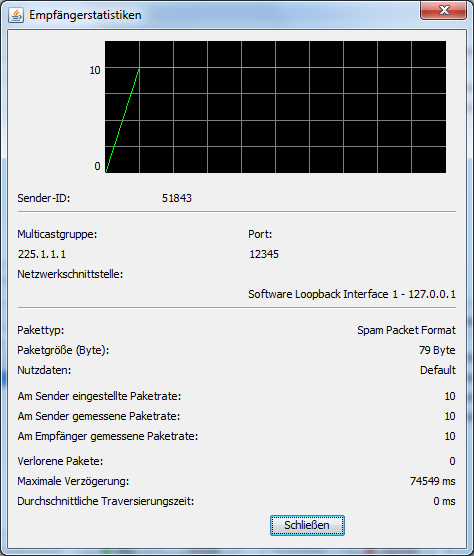
\includegraphics[width=11cm]{images/showEmpfaenger.png}
\caption[Empfängerstatistiken]{Empfängerstatistiken}
\label{receiverstatistics}
\end{center}
\end{figure}

Innerhalb dieses Dialogfensters werden verschiedene Statistiken, allgemeine
Informationen zum Empfänger, sowie ein Graph, welcher den Verlauf der Paketrate
darstellt, angezeigt.

\newpage
\begin{table}[h]
\caption{Daten - Empfängerstatistiken}
\label{tab:showEmpfaenger}
\begin{center}
\begin{tabular}{|p{6cm}|p{8cm}|}
\hline
\textbf{Bezeichnung} & \textbf{Beschreibung}\\
\hline
Graph & Zeigt grafisch den Verlauf der gemessenen Paketrate\\
\hline
Sender-ID & Zeigt die Sender-ID an\\
\hline
Multicastgruppe & Zeigt die Multicastgruppe, an die gesendet wird.\\
\hline
Port & Zeigt den Port, an den gesendet wird\\
\hline
Pakettyp & Zeigt den verwendeten Pakettypen\\
\hline
Paketgröße & Zeigt die definierte Paketgröße\\
\hline
Nutzdaten & Zeigt die definierten Nutzdaten\\
\hline
Am Sender eingestellte Paketrate & Zeigt die eingestellte Paketrate am Sender\\
\hline
Am Sender gemessene Paketrate & Zeigt die gemessene Paketrate am Sender\\
\hline
Am Empfänger gemessene Paketrate & Zeigt die gemessene Paketrate am Empfänger\\
\hline
Verlorene Pakete & Zeigt die Anzahl der verlorenen Pakete\\
\hline
Maximale Verzögerung & Zeigt die maximale Verzögerung zwischen zwei Paketen\\
\hline
Durchschnittliche Traversierungszeit & Zeigt die durchschnittliche
Traversierungszeit\\
\hline
\end{tabular}
\end{center}
\label{default}
\end{table}

\chapter{Menü}
Durch Klicken auf das Feld ``Datei'' in der Menüleiste des Hauptfensters öffnet
sich ein Menü. Dieses Menü enthält Einträge zum Öffnen von Dialogen für das
Laden und Speichern eines Profils, für Einstellungen zum Ändern der Sprache,
eine Liste bekannter zuletzt verwendeter Profile, sowie einen Eintrag zum
Beenden des Multicast Tools.

\begin{figure}[htbp]
\begin{center}
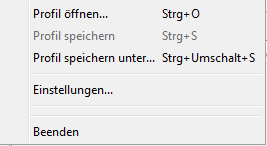
\includegraphics{images/menu1.png}
\caption[Menü]{Menü}
\label{menu1}
\end{center}
\end{figure}

Durch Klicken auf eines der bekannten Profile in der Liste wird dieses sofort
geladen, d.h. alle Sender und Empfänger werden so angelegt, wie es in dem Profil
spezifiziert ist.

\begin{figure}[htbp]
\begin{center}
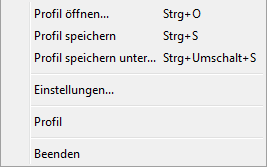
\includegraphics{images/menu2.png}
\caption[Menü mit bekannten Profilen]{Menü mit bekannten Profilen}
\label{menu2}
\end{center}
\end{figure}

\chapter{Profil Speichern\ldots}
Durch Klicken auf ``Profil speichern unter\ldots'' oder durch Drücken der
Tastenkombination ``STRG+Umschalt+S'' wird das Dialogfenster zum Speichern eines
Profils aufgerufen.

\begin{figure}[htbp]
\begin{center}
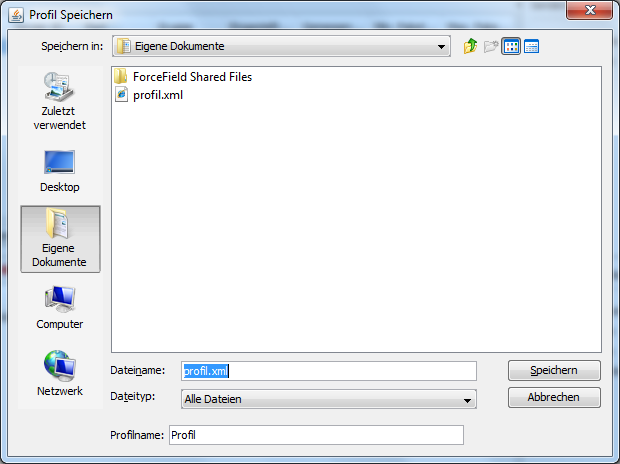
\includegraphics[width=14cm]{images/saveProfile.png}
\caption[Profil speichern]{Profil speichern}
\label{saveprofile}
\end{center}
\end{figure}

Das Dialogfenster zum Speichern eines Profils besteht aus einem Bereich zum
auswählen des Speicherortes, einem Eingabefeld zur Eingabe eines Dateinamens
sowie einem weiteren Eingabefeld zur Eingabe eines Profilnamens. Dieser
Profilname wird in der Liste der bekannten/zuletzt verwendeten Profile
angezeigt, sowie nach erfolgreichem Laden in der Titelleiste des Hauptfensters.

\chapter{Profil öffnen\ldots}
Durch Klicken auf  ``Profil öffnen\ldots'' im Menü oder durch Drücken der
Tastenkombination ``STRG+O'' wird das Dialogfenster zum Öffnen/Laden eines
Profils aufgerufen. 

\begin{figure}[htbp]
\begin{center}
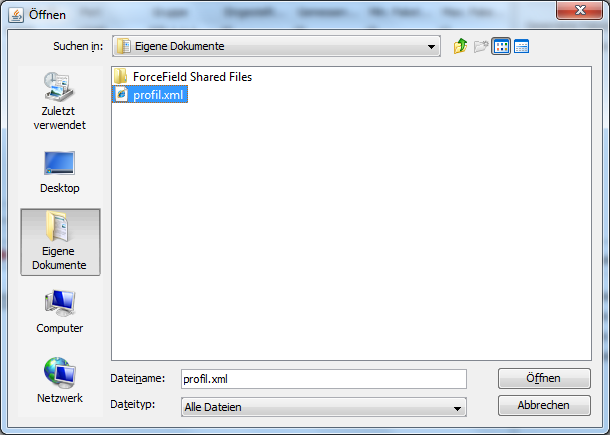
\includegraphics[width=14cm]{images/openProfile.png}
\caption[Profil öffnen]{Profil öffnen}
\label{openprofile}
\end{center}
\end{figure}

Dieses Dialogfenster besteht aus einem Bereich zum auswählen der Datei. Durch
Bestätigen wird das Profil geladen und alle bisher vorhandenen Sender/Empfänger
werden entfernt.

\chapter{Einstellungen\ldots}
Durch Klicken auf ``Einstellungen\ldots'' im Menü wird das Dialogfenster zum
Ändern von Einstellungen (in der aktuellen Version nur Sprache) angezeigt. 

\begin{figure}[htbp]
\begin{center}
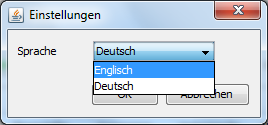
\includegraphics{images/options.png}
\caption[Einstellungen]{Einstellungen}
\label{options}
\end{center}
\end{figure}

Durch Auswählen einer Sprache aus dem Ausklapp-Menü sowie Bestätigung wird die
entsprechende Sprache angewendet.

\chapter{Commandline Interface}
Neben der Bedienung mittels der grafischen Benutzeroberfläche ist es auch
möglich das MulticastTool via Kommandozeile zu bedienen.
Die folgende Tabelle ist eine Auflistung der Befehle sowie ihrer
Bedeutung.

\begin{table}[h]
\caption{CLI Befehle}
\label{tab:cli}
\begin{center}
\begin{tabular}{|p{6cm}|p{8cm}|}
\hline
\textbf{Befehl} & \textbf{Beschreibung}\\
\hline
-nogui & Startet das Tool ohne GUI\\
\hline
-cli & Startet den Logger mit\\
\hline
-profile <PROFILNAME> & Lädt ein oder mehrere Profile anhand des
Profilnamens (getrennt durch Leerzeichen)\\
\hline
-path <PATH> & Lädt ein oder mehrere Profile anhand eines Pfades (getrennt durch
Leerzeichen)\\
\hline
-startall & Startet alle Sender/Empfänger der geladenen Konfigurationen\\
\hline
-startnone & Startet keine der Sender/Empfänger der geladenen Konfigurationen\\
\hline
-restore & Startet alle Sender/Empfänger in dem Status (aktiv/inaktiv), wie im
Profil gespeichert (default)\\
\hline
\end{tabular}
\end{center}
\label{default}
\end{table}